\documentclass[]{book}

%These tell TeX which packages to use.
\usepackage{array,epsfig}
\usepackage{amsmath}
\usepackage{amsfonts}
\usepackage{amssymb}
\usepackage{amsxtra}
\usepackage{amsthm}
\usepackage{mathrsfs}
\usepackage{color}
\usepackage[margin=2cm,top=2.5cm,headheight=16pt,headsep=0.1in,heightrounded]{geometry}
\usepackage{fancyhdr}
\pagestyle{fancy}
\usepackage{tikz}
\usepackage{graphics}
\usepackage{float}

%Here I define some theorem styles and shortcut commands for symbols I use often
\theoremstyle{definition}
\newtheorem{defn}{Definition}
\newtheorem{thm}{Theorem}
\newtheorem{cor}{Corollary}
\newtheorem*{rmk}{Remark}
\newtheorem{lem}{Lemma}
\newtheorem*{joke}{Joke}
\newtheorem{ex}{Example}
\newtheorem*{soln}{Solution}
\newtheorem{prop}{Proposition}

\newcommand{\lra}{\longrightarrow}
\newcommand{\ra}{\rightarrow}
\newcommand{\surj}{\twoheadrightarrow}
\newcommand{\graph}{\mathrm{graph}}
\newcommand{\bb}[1]{\mathbb{#1}}
\newcommand{\Z}{\bb{Z}}
\newcommand{\Q}{\bb{Q}}
\newcommand{\R}{\bb{R}}
\newcommand{\E}{\bb{E}}
\newcommand{\C}{\bb{C}}
\newcommand{\N}{\bb{N}}
\newcommand{\Pe}{\bb{P}}
\newcommand{\M}{\mathbf{M}}
\newcommand{\m}{\mathbf{m}}
\newcommand{\MM}{\mathscr{M}}
\newcommand{\HH}{\mathscr{H}}
\newcommand{\Om}{\Omega}
\newcommand{\Ho}{\in\HH(\Om)}
\newcommand{\bd}{\partial}
\newcommand{\del}{\partial}
\newcommand{\bardel}{\overline\partial}
\newcommand{\textdf}[1]{\textbf{\textsf{#1}}\index{#1}}
\newcommand{\img}{\mathrm{img}}
\newcommand{\ip}[2]{\left\langle{#1},{#2}\right\rangle}
\newcommand{\inter}[1]{\mathrm{int}{#1}}
\newcommand{\exter}[1]{\mathrm{ext}{#1}}
\newcommand{\cl}[1]{\mathrm{cl}{#1}}
\newcommand{\ds}{\displaystyle}
\newcommand{\vol}{\mathrm{vol}}
\newcommand{\cnt}{\mathrm{ct}}
\newcommand{\osc}{\mathrm{osc}}
\newcommand{\LL}{\mathbf{L}}
\newcommand{\UU}{\mathbf{U}}
\newcommand{\support}{\mathrm{support}}
\newcommand{\AND}{\;\wedge\;}
\newcommand{\OR}{\;\vee\;} 
\newcommand{\Oset}{\varnothing}
\newcommand{\st}{\ni}
\newcommand{\wh}{\widehat}
\newcommand{\vect}[1]{\overrightarrow{#1}}

%Pagination stuff.
%\setlength{\oddsidemargin}{0in}
%\setlength{\evensidemargin}{0in}
\setlength{\textheight}{9.in}
\setlength{\textwidth}{6.5in}
\cfoot{page \thepage}
\lhead{MEU359 - Proba-Stat}
\rhead{TP}
\pagestyle{fancy}


\begin{document}

\subsection*{Question 1}
On voit clairement sur le nuage de points (circonference/hauteur) que cela suit une droite. On essaye de trouver les valeurs de la droites qui minimisent le risque quadratique.

\subsection*{Question 2}
Pour minimiser la fonction $\varphi(\beta_1, \beta_2)$ il faut trouver d\'eriver la fonction par rapport \`a $\beta_1$ et $\beta_2$ et trouver les valeurs qui annulent les 2 d\'eriv\'ees.
$$
\frac{\partial \varphi(\beta_1, \beta_2)}{\beta_1} = \frac{\sum_{i=1}^{n}{(Y_i - \beta_1 - \beta_2x_i)^2}}{\beta_1} = \frac{\sum_{i=1}^{n}{Y_i^2 - \beta_1Y_i - \beta_2x_iY_i -\beta_1Y_i + \beta_1^2 + \beta_1\beta_2x_i - \beta_2x_iY_i + \beta_2x_i\beta_1 +\beta_2^2x_i^2}}{\beta_1}
$$
$$
= \sum_{i=1}^{n}{-Y_i -Y_i +2\beta_1 +\beta_2x_i+\beta_2x_i} = 2 \sum_{i=1}^{n}{-Y_i+\beta_2x_i+\beta_1}
$$
$$
\frac{\partial \varphi(\beta_1, \beta_2)}{\beta_2} = \frac{\sum_{i=1}^{n}{(Y_i - \beta_1 - \beta_2x_i)^2}}{\beta_2} = \frac{\sum_{i=1}^{n}{Y_i^2 - \beta_1Y_i - \beta_2x_iY_i -\beta_1Y_i + \beta_1^2 + \beta_1\beta_2x_i - \beta_2x_iY_i + \beta_2x_i\beta_1 +\beta_2^2x_i^2}}{\beta_2}
$$
$$
= \sum_{i=1}^{n}{-x_iY_i+\beta_1x_i-x_iY_i + \beta_1x_i+2\beta_2x_i^2} = 2 \sum_{i=1}^{n}{x_i(-Y_i+\beta_2x_i+\beta_1)}
$$

On cherche $\hat{\beta_1}$ et $\hat{\beta_2}$ les valeurs qui annulent le syst\`eme
$$
\left\{
\begin{array}{l}
\sum_{i=1}^{n}{x_i(-Y_i+\beta_2x_i+\beta_1)} = 0 \\
\sum_{i=1}^{n}{-Y_i+\beta_2x_i+\beta_1} = 0
\end{array}
\right.
$$
$$
\left\{
\begin{array}{l l}
\sum_{i=1}^{n}{-Y_ix_i}+\sum_{i=1}^{n}{\beta_2x_i^2}+\sum_{i=1}^{n}{\beta_1x_i} = 0 & (1)\\
\sum_{i=1}^{n}{-Y_i} +\sum_{i=1}^{n}{\beta_2x_i}+\sum_{i=1}^{n}{\beta_1} = 0 & (2)
\end{array}
\right.
$$
$$
\left\{
\begin{array}{l l}
\sum_{i=1}^{n}{-Y_ix_i}+\beta_2\sum_{i=1}^{n}{x_i^2}+\beta_1\sum_{i=1}^{n}{x_i} = 0 & (1)\\
\sum_{i=1}^{n}{-Y_i} +\beta_2\sum_{i=1}^{n}{x_i}+n\beta_1 = 0 & (2)
\end{array}
\right.
$$



On fait $(3) = n(1)-(2)\sum_{i=1}^{n}{x_i}$
$$
\left\{
\begin{array}{l l}
n\sum_{i=1}^{n}{-Y_ix_i}+n\beta_2\sum_{i=1}^{n}{x_i^2}+\sum_{i=1}^{n}{Y_i}\sum_{i=1}^{n}{x_i} -\beta_2\left(\sum_{i=1}^{n}{x_i}\right)^2 = 0 & (3)\\
\sum_{i=1}^{n}{-Y_i} +n\beta_2\sum_{i=1}^{n}{x_i}+n\beta_1 = 0 & (2)
\end{array}
\right.
$$
$$
\left\{
\begin{array}{l l}
-n\sum_{i=1}^{n}{Y_ix_i} + \sum_{i=1}^{n}{Y_i}\sum_{i=1}^{n}{x_i} = \beta_2\left(\sum_{i=1}^{n}{x_i}\right)^2 -n\beta_2\sum_{i=1}^{n}{x_i^2}  & (3)\\
\sum_{i=1}^{n}{-Y_i} +n\beta_2\sum_{i=1}^{n}{x_i}+n\beta_1 = 0 & (2)
\end{array}
\right.
$$
$$
\left\{
\begin{array}{l l}
\beta_2 = \frac{\sum_{i=1}^{n}{Y_i}\sum_{i=1}^{n}{x_i}-n\sum_{i=1}^{n}{Y_ix_i}}{\left(\sum_{i=1}^{n}{x_i}\right)^2 -n\sum_{i=1}^{n}{x_i^2}}  & (3)\\
\beta_1 = \frac{1}{n}(\sum_{i=1}^{n}{Y_i} - n\beta_2\sum_{i=1}^{n}{x_i}) & (2)
\end{array}
\right.
$$
$$
\left\{
\begin{array}{l l}
\beta_2 = \frac{\sum_{i=1}^{n}{Y_i}\sum_{i=1}^{n}{x_i}-n\sum_{i=1}^{n}{Y_ix_i}}{\left(\sum_{i=1}^{n}{x_i}\right)^2 -n\sum_{i=1}^{n}{x_i^2}}  & (3)\\
\beta_1 = \frac{\sum_{i=1}^{n}{x_i}\sum_{i=1}^{n}{x_iY_i}-\sum_{i=1}^{n}{x_i^2}\sum_{i=1}^{n}{Y_i}}{\left(\sum_{i=1}^{n}{x_i}\right)^2 -n\sum_{i=1}^{n}{x_i^2}} & (2)
\end{array}
\right.
$$

\subsection*{Question 3}
Voir Python.
\begin{figure}
	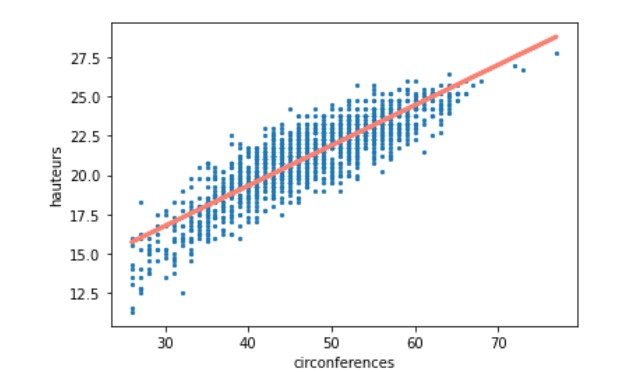
\includegraphics[scale=1]{regression_simple.jpg}
    \caption{Regression simple}
    \label{fig:regression simple}
\end{figure}

On obtient $\beta_1 =  9.037475668452768$  et $\beta_2 = 0.257137855007109$.

\subsection*{Question 4}
Comme le montre les figures 2 et 3, il semble raisonnable de dire que la circonf\'erence (resp. la hauteur) d'un eucalyptus suit une loi normale. Maintenant on n'a qu'un seul \'echantillon, donc cela pourrait \^etre une pure coincidence!

\begin{figure}
    \centering
    \begin{minipage}{0.45\textwidth}
        \centering
            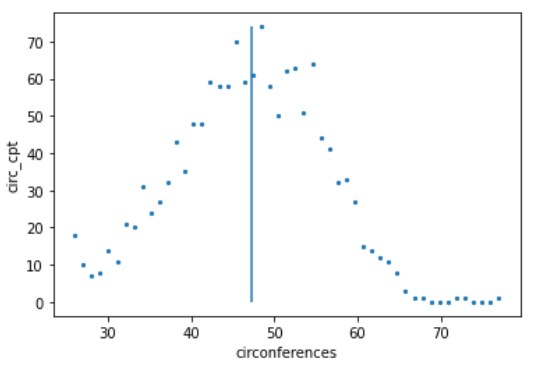
\includegraphics[scale=0.5]{circ_normale.jpg}
            \caption{Circonference}
            \label{fig:Circonference}
    \end{minipage}\hfill
    \begin{minipage}{0.45\textwidth}
        \centering
        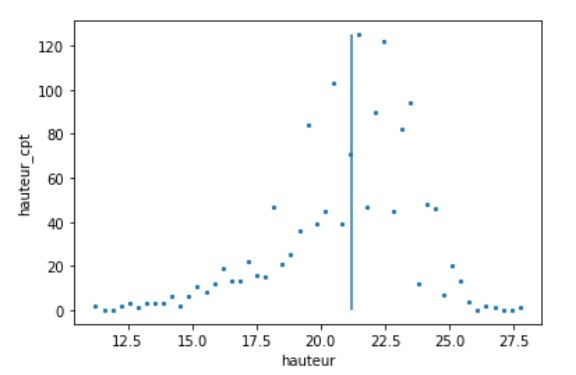
\includegraphics[scale=0.5]{hauteur_normale.jpg}
        \caption{Hauteur}
        \label{fig:Hauteur}
    \end{minipage}
\end{figure}


Comme les 2 variables al\'eatoire suivent une loi normale, elle sont ind\'ependentes et identiquement distribu\'es.

Si X suit une loi normale $\mathscr{N}(m, \sigma^2)$ et $Y = AX + b$ alors, $Y$ suit une loi normale $\mathscr{N}(am + b, a^2\sigma^2)$  

Si $X$ (resp. $Y$) suit une loi normale $\mathscr{N}(m_x, \sigma_x^2)$ (resp. $\mathscr{N}(m_y, \sigma_y^2)$) alors $X+Y$ suit une loi normale $\mathscr{N}(m_x + m_y, \sigma_x^2+\sigma_y^2)$.

Dans notre cas on a $e_i = Y_i - \hat{\beta_1} + \hat{\beta_2}x_i$. Donc $e_i$ suit une loi normale  
$\mathscr{N}(- \hat{\beta_1} - \hat{\beta_2}m_x + m_Y, \hat{\beta_2}^2\sigma_x^2+\sigma_y^2)$. On a par d\'efinition $m_y = \hat{\beta_1} + \hat{\beta_2}m_x$. Donc $E(e_i) = 0$ et $\sigma_{e_i} = \hat{\beta_2}^2\sigma_x^2+\sigma_y^2$.


\subsection*{Question 5}
En cherchant \`a minimiser $\lVert Y - X\beta \rVert^2$, on cherche \`a trouver l'\'el\'ement de $F$ le plus proche de $Y$ au sens de la distance euclidienne. Il s'agit de la projection orthogonale de $Y$ sur $F$. Comme $z \in F$, si et seulement si $z = X\beta$, on cherche $\hat{\beta}$ tel que $X\hat{\beta} = P_F(Y)$. 

Comme $X\hat{\beta} = P_F(Y)$, on a $Y - X\hat{\beta} = Y - P_F(Y)$ qui est un vecteur orthogonal \`a $X$ et par cons\'equent aussi a $X\theta$. Le produit scalaire de 2 vecteurs orthogonaux est nul, donc $\forall \theta \in \R^{3} <Y - X\hat{\beta}, X\theta> = 0$.

\subsection*{Question 6}
Pour trouver le minimum par rapport a $\beta$, il suffit de d\'eriver l'expression par rapport \`a $\beta$ et annuler l'expression. On remarque que $\sum_{i=1}^{n}{(Y-X\beta)^2} = (Y-X\beta)^t(Y-X\beta)$

$$
(Y-X\beta)^t(Y-X\beta) = (Y^t-\beta^tX^t)(Y-X\beta) = Y^tY-Y^tX\beta - \beta^tX^tY + \beta^tX^tX\beta
$$
et
$$
\frac{\partial (Y-X\beta)^t(Y-X\beta) }{\partial \beta} = -Y^tX + \beta^tX^tX
$$
On cherche $\hat{\beta}$ tel que
$$
-Y^tX + \hat{\beta}^tX^tX = 0
$$
$$
(\hat{\beta}^tX^tX)^t = (-Y^tX)^t
$$
Donc
$$
\hat{\beta} = (X^tX)^{-1}X^tY
$$

\subsection*{Question 7}
Voir Python.

\begin{figure}
	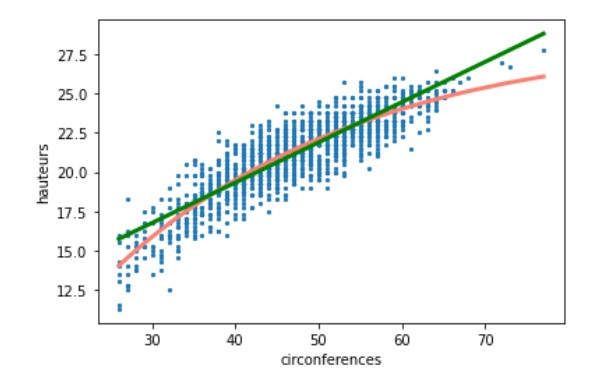
\includegraphics[scale=1]{regression_multiple.jpg}
    \caption{Regression multiple}
    \label{fig:Regression multiple}
\end{figure}

$$\beta = [-24.35200327,  -0.48294547,   9.98688814]$$

\subsection*{Question 8}
On a $Y = X\beta + \epsilon$. On suppose que les variables al\'eatoires $\epsilon_i$ suivent une loi normale $\mathscr{N}(0,\sigma^2)$. On ne sait rien de la loi de la variable al\'eatoire $X$, donc on ne peut rien dire sur la loi des $Y_i$. En effet, supposons que la variable al\'eatoire $X$ suit une loi exponentielle, alors $Y_i$ suivra probablement une loi exponentielle.

Maintenant, sur le seul \'echantillon fourni, on a montr\'e \`a la question 4 que $Y_i$ suit certainement une loi normale.

Au vu du nuage de points, pourquoi ne pas prendre $Y = \beta_1 + \beta_2x_i + \beta_3x_i^2 + \beta_3x_i^3 + \beta_4x_i^4$? Meilleure courbe. Et surement meilleur si on prend un ordre 10 ou 30.

??? pour le reste.

\subsection*{Test de Student}
Pourquoi on cherche \`a se demander si $\beta_3 = 0$. On suppose ici que les $\beta_1$ et $\beta_2$ sont identiques pour les 2 r\'egressions pour l'\'echantillon donn\'e. Ce qui n'est pas le cas.

\subsection*{Question 9}
Soient Z une variable al\'eatoire de loi normale centr\'ee et r\'eduite et U une variable ind\'ependante de Z et distribu\'ee suivant la loi la loi du chi-deux \`a k degr\'es de libert\'e. Par d\'efinition la variable $T=\frac {Z}{\sqrt {U/k}}$ suit une loi de Student \`a k degr\'es de libert\'e.

Prenons $U = (n-3)\frac{\hat{\sigma}^2}{\sigma^2}$ et $Z = \hat{\beta}_3$. On sait que $U$ suit une loi de chi-deux \`a $(n-3)$ degr\'es de libert\'e (voir question pr\'ec\'edente) et que $Z$ suit une loi normale centr\'ee et r\'eduite. Donc

$$
T = \frac{\hat{\beta}_3}{\sqrt{\frac{(n-3)\frac{\hat{\sigma}^2}{\sigma^2}}{n-3}}} = \frac{\hat{\beta}_3}{\frac{\hat{\sigma}}{\sigma}} = \frac{\hat{\beta}_3\sigma}{\hat{\sigma}}
$$





\end{document}

